\documentclass[5p,authoryear]{elsarticle}
\usepackage{mathtools}
\usepackage{amsmath}
\usepackage{graphicx}
\usepackage{times}
\usepackage{amssymb}
\usepackage{multirow}
\setlength{\topmargin}{-1.25cm}
% \voffset -2.0cm

% --- macros --- %
\newcommand{\hompc}{\,h\,{\rm Mpc}^{-1}}
\newcommand{\mpcoh}{\,h^{-1}\,{\rm Mpc}}
\newcommand{\cell}[1]{\multirow{2}{*}{#1}}

% --- document --- %
\begin{document}

% --- title --- %
\title{PICOLA: A new code for generating large ensembles of dark matter realizations}

\author[icg]{Cullan Howlett\corref{email1}}
\author[icg,ucl]{Marc Manera}
\author[icg]{Will Percival}
\address[icg]{Institute of Cosmology \& Gravitation, Dennis Sciama Building, University of Portsmouth, Portsmouth, PO1 3FX, UK}
\address[ucl]{ENTER UCL ADDRESS HERE...}
\cortext[email1]{cullan.howlett@port.ac.uk}
\date{outline} 

\begin{abstract}
Detailed analysis of current large-scale structure surveys calls for large numbers of realistic mock galaxy catalogues that mimic the observed distribution of galaxies within the survey volume. Such an ensemble of mock catalogues can be used to pin down statistical and systematic errors in survey data and help to shape the design of future surveys, by allowing rigourous examination of survey design, data reduction pipelines, and possible cosmological inferences. As large-scale structure surveys enter into a new era of precision, sub-percent, cosmology, we find that both the accuracy and sheer amount of mock galaxy catalogues must also increase. To this end we present a new, fast, planar-parallel code, {\sc picola}, which can be used to generate and evolve a set of initial conditions into a dark matter field. Through comparisons to N-Body simulations we find that our code can replicate the observed clustering of dark matter to \textbf{ACCURATE TO WHAT?} and halos to \textbf{ACCURATE TO WHAT?}, \textbf{XXXX: Mention something about it being better than other methods}, but orders of magnitude faster than a standard N-Body run. 
\end{abstract} 

\begin{keyword}
\end{keyword}

\maketitle

\section{Introduction}
Understanding the nature of our universe and its fundamental components through the statistical analysis of the large scale distribution of galaxies has been an increasingly active area of research over the last 30 years. In particular, the first clear (>3.0$\sigma$) detection of the Baryon Acoustic Oscillation (BAO) feature in the 3-D distribution of galaxies by both the SDSS-II \citep{Eisenstein:2005} and 2dF \citep{Cole:2005} surveys nearly a decade ago means that we can now constrain the evolution of our universe to greater precision than ever before. In order to accurately determine cosmological parameters and distinguish between different cosmological models we require that systematic errors in our measurements are known to a high precision and that our knowledge of the statistical errors, in the form of the covariance matrix, is as complete as possible. We can measure both of these using mock galaxy catalogues, which mimic our real survey as closely as possible, by applying potential systematics to the catalogues themselves and by producing a large number of realisations to compute the covariance matrix, such that we reduce the noise due to cosmic variance.



Need for Mock catalogues, cite BOSS, WiggleZ, 2df \\
Other methods for producing mocks (PTHalos, PINOCCHIO, QPM) \\
Overview of the paper.

\section{The COmoving Lagrangian Acceleration (COLA) method}

In the following section we reinterate the  COLA method for evolving a system of dark matter particles under gravity, as first introduced by \cite{Tassev2013}. We begin with a summary of the theoretical underpinnings of the algorithm, including a brief overview of second order langrangian perturbation theory (2LPT), before moving onto the algorithmic implementation.

\subsection{2LPT}
As described in \cite{Scoccimarro1998} (see also \cite{Moutarde1991} and \cite{Bouchet1995}), cold dark matter particles evolving over cosmological time in an expanding universe follow the equation of motion
\begin{equation}
\frac{d^{2}\boldsymbol{\Psi}}{d\tau^{2}} + \mathcal{H}(\tau)\frac{d\boldsymbol{\Psi}}{d\tau} + \nabla \Phi = 0,
\label{eom}
\end{equation}
where $\Phi$ is the gravitational potential, $\mathcal{H}(\tau) = \frac{dlna}{d\tau}$ is the conformal Hubble parameter and $a$ is the scale factor. $\boldsymbol{\Psi}$ is the displacement vector of the particle and relates the particle's Eulerian position $\boldsymbol{x}(\tau)$ to its initial, Lagrangian position, $\boldsymbol{q}$, via
\begin{equation}
\boldsymbol{x}(\tau) = \boldsymbol{q} + \Psi(\boldsymbol{q},\tau).
\label{lagrangian}
\end{equation}
By taking the divergence of the equation of motion and using the poisson equation, we find
\begin{equation}
\nabla_{x} \cdot \left( \frac{d^{2}\boldsymbol{\Psi}}{d\tau^{2}} + \mathcal{H}(\tau)\frac{d\boldsymbol{\Psi}}{d\tau} \right) = - \frac{3}{2} \Omega_{m}. \mathcal{H} \delta
\label{eom2}
\end{equation}
Lagrangian perturbation theory seeks to solve (\ref{eom2}) by perturbatively expanding the displacement vector,
\begin{equation}
\boldsymbol{\Psi} = \boldsymbol{\Psi}^{(1)} + \boldsymbol{\Psi}^{(2)} + \ldots,
\end{equation}
If we then apply the continuity equation, $\rho(\boldsymbol{x},t)d^{3}x = \rho(\boldsymbol{q},0)d^{3}q$, which states that a mass element $d^{3}q$ centred at $\boldsymbol{q}$ at time zero becomes a mass element $d^{3}x$, centred at $\boldsymbol{x}$, at time $t$, we find that, to first order
\begin{equation}
\nabla_{q} \cdot \boldsymbol{\Psi}^{(1)} = -D_{1}(\tau) \delta_{L}(\boldsymbol{q}).
\label{za}
\end{equation}
Here $D_{1}(\tau)$ is the linear growth factor, $\delta_{L}(q)$ is the linear overdensity field and we have rewritten the divergence as a function of $\boldsymbol{q}$ by using the fact that they are related via the Jacobian of the transformation from $\boldsymbol{x}$ to $\boldsymbol{q}$, i.e., $\nabla x_{i} = (\delta_{ij} + \partial \boldsymbol{\Psi}_{i}/\partial \boldsymbol{q}_{j})^{-1} \nabla q_{j}$.
Solving to second order introduces corrections to the first order displacement of the form
\begin{equation}
\nabla_{q} \cdot \boldsymbol{\Psi}\,^{(2)}= \frac{1}{2}D_{2}(\tau)\sum_{i\neq j}\left(\boldsymbol{\Psi}^{(1)}_{i,i}\boldsymbol{\Psi}^{(1)}_{j,j} - \boldsymbol{\Psi}^{(1)}_{i,j}\boldsymbol{\Psi}^{(1)}_{j,i} \right),
\label{2lpt}
\end{equation}
where, for brevity, we have defined $\boldsymbol{\Psi}_{i,j}=\partial \boldsymbol{\Psi}_{i}/\partial \boldsymbol{q}_{j}$.
\cite{Bouchet1995} provide a good approximation for $D_{2}(\tau)$, the second order growth factor, for a flat universe with non-zero cosmological constant
\begin{equation}
D_{2}(\tau) \approx -\frac{3}{7}D^{2}_{1}(\tau)\Omega_{m}(\tau)^{-1/143}. 
\end{equation}
For further computational ease, we can define two Langragian potentials, $\boldsymbol{\Psi}^{(i)}=\nabla_{q}\phi^{(i)}$, such that (\ref{lagrangian}) becomes
\begin{equation}
\boldsymbol{x}(\tau) = \boldsymbol{q} - D_{1}\nabla_{q}\phi^{(1)} + D_{2}\nabla\phi^{(2)},
\end{equation}
and the Lagrangian potentials are obtained by solving the corresponding pair of Poisson equations derived from (\ref{za}) and (\ref{2lpt}) respectively
\begin{equation}
\nabla_{q}^{2}\phi^{(1)} = \delta_{L}(\boldsymbol{q}).
\end{equation}
\begin{equation}
\nabla_{q}^{2}\phi^{(2)} =\sum_{i>j}\left(\phi_{i,i}^{(1)}\phi_{j,j}^{(1)} - (\phi_{i,j}^{(1)})^{2}\right).
\end{equation}

\subsection{COLA}
The COLA method \citep{Tassev2013} provides a much more accurate solution to Eq. (\ref{eom}) than 2LPT, at only a moderate ($\sim 3\times$) reduction in speed. It does this by utilising the first and second-order Langrangian displacements, which provide an exact solution at large, quasi-linear scales, and solving for the resultant, non-linear component. By switching to a frame of reference comoving with the particles in Lagrangian space, we can split the dark matter equation of state as follows,
\begin{equation}
T[\boldsymbol{\Psi}_{res}]+ T[{D}_{1}]\boldsymbol{\Psi}_{1} + T[{D}_{2}]\boldsymbol{\Psi}_{2} + \nabla \Phi = 0,
\end{equation}
where,
\begin{equation}
T[X] = \frac{d^{2}X}{d\tau^{2}} + \mathcal{H}\frac{dX}{d\tau}.
\end{equation}
$\boldsymbol{\Psi}_{res}$ is the remaining displacement when we subtract the quasi-linear 2LPT displacements from the full, non-linear displacement each particle should actually feel. 

The reason this method is so useful is because we only need to calculate the Lagrangian displacements once, at redshift $z=0$, and scale them by the appropriate derivatives of the growth factor. In fact, as we will see in later sections,  it is common practice in many N-Body simulations to use 2LPT to generate the initial positions of the particles at a suitably high redshift, where the results are exact. In terms of implementing COLA all this means is that we need to store the 2LPT displacements after we use them to set up the initial conditions of our simulation. Implementing the bridge between the 2LPT and COLA methods, switching to a Lagrangian frame of reference, is then as simple as removing the particle's initial 2LPT velocity and  adding it back on at the end of the simulation when we revert back to our original frame of reference.

The only addition that requires extra computation is solving for the residual displacement, $\boldsymbol{\Psi}_{res}$. In the COLA method this is done using the well-known Particle-Mesh algorithm.

\subsection{Particle-Mesh algorithm}

Here we provide a brief overview of the Particle-Mesh (PM) algorithm (see \cite{Hockney1982} for a good review of this method). Our implementation is based on the publicly available {\sc pmcode}\footnote{http://astro.nmsu.edu/~aklypin/PM/pmcode/}, and as such we refer the reader to the associated documentation for full details on the set of equations we solve to get the displacement. 

In the PM method we place a mesh over our dark matter particles and solve for the gravitational forces at each mesh point. We then interpolate to find the force at the position of each particle and use this to calculate the displacement each particle receives. This is performed iteratively over a series of small timesteps. For $N_{m}^{3}$ mesh points and $N^{3}$ particles, this means that at each iteration we only need to perform $N_{m}$ force calculations, which is much faster than a direct summation of the contribution to the gravitational force from each individual particle (at least for all practical applications, where $N \approx N_{m}$). 

At each iteration we perform the following steps to calculate the displacement:
\begin{enumerate}
\item{Use the Cloud-in-cell linear interpolation method to assign the particles to the mesh, thereby calculating the mass density, $\rho(\boldsymbol{x})$, at each mesh point.}
\item{Use a Fast Fourier Transform (FFT)\footnote{In all cases we use the FFTW-3 Discrete Fourier Transform routines to compute our Fourier transforms. This library is freely available from http://www.fftw.org/} to Fourier transform the density and solve the comoving Poisson equation in Fourier space.}
\begin{equation}
k^2 \phi(\boldsymbol{k}) =  \frac{3}{2}\frac{\Omega_{m,0}}{a}(\rho(\boldsymbol{k})-1)
\end{equation}
\item{Use the gravitational potential and an Inverse-FFT to generate the force in each direction in real-space. Here we also deconvolve the Cloud-in-cell window function.}
\begin{equation}
F(\boldsymbol{k}) = \boldsymbol{k}\phi(\boldsymbol{k})
\end{equation}
\item{Calculate the acceleration each particle receives in each direction, again using the Cloud-in-cell interpolation method to interpolate from the mesh points.}
\end{enumerate}

\subsection{Timestepping}

Once we have calculated the acceleration, we combine this with the first and second order Lagrangian Displacements and use the Kick-Drift-Kick/Leapfrog Method \citep{Quinn1998} to update the particle velocities and positions. Here, particle velocities are calculated from the displacements and updated to the nearest half-integer timestep. The particle positions are then updated to the nearest integer timestep using the previous velocity. In this way the particle velocities and positions are never (except at the beginning and end) calculated for the same point in time but rather 'leapfrog' over each other with the next iteration of the velocity dependent on the position from the previous iteration and so on. 
\begin{align}
&\boldsymbol{v}_{i+1/2} = \boldsymbol{v}_{i-1/2} - T[\boldsymbol{\Psi}_{res}]\Delta a_{1}, \\
&\boldsymbol{r}_{i+1} = \boldsymbol{r}_{i} + \boldsymbol{v}_{i+1/2}\Delta a_{2} + \Delta D_{1}\boldsymbol{\Psi}_{1} + \Delta D_{2}\boldsymbol{\Psi}_{2}
\end{align}
Here $\Delta D = D_{i+1} - D_{i}$ denotes the change in the first and second order growth factors over the timestep and $\Delta a$ encapsulates the time interval and appropriate numerical factors required to convert the displacement to a velocity and the velocity to a position. There are several choices for how we calculate $\Delta a$ for each timestep. Using the standard method from \cite{Quinn1998}, we can evaluate these, for the COLA method, as
\begin{align}
\Delta a_{1} &= \frac{H_{0}}{a_{i}}\int_{a_{i-1/2}}^{a_{i+1/2}} \frac{da}{a^{2}H(a)}, \notag \\
\Delta a_{2} &= H_{0}\int_{a_{i}}^{a_{i+1}}\frac{da}{a^{3}H(a)}.
\end{align}
However, \cite{Tassev2013} present a second, COLA specific, formulation which gives faster convergence, hence allowing us to recover our evolved dark matter field to greater accuracy in fewer time steps. In their method,
\begin{align}
\Delta a_{1} &= \frac{H_{0}}{nLPT}\frac{a_{i+1/2}^{nLPT}-a_{i-1/2}^{nLPT}}{a_{i}^{nLPT-1}}, \notag \\
\Delta a_{2} &= \frac{H_{0}}{a_{i+1/2}^{nLPT}}\int_{a_{i}}^{a_{i+1}}\frac{a^{nLPT-3}}{H(a)} da.
\end{align}
where they find the best results using a value $nLPT=2.5$. As the choice of timestepping method is somewhat arbitrary {\sc picola} retains both methods as options. Hence, whilst hard-coded and unable to be changed at run-time, the choice of timestepping method (and $nLPT$) should still be treated formally as an extra degree of freedom in the code. 

\section{A Parallel Implementation of COLA (PICOLA)}

We have designed {\sc picola} to be a stand alone code in the sense that we can generate a dark matter realisation based solely on a small number of user defined parameters. This includes calculating the initial linear dark matter power spectrum (although {\sc picola} also accepts an input file containing this), generating an initial particle distribution with k-space distribution that matches this power spectrum, and evolving the dark matter field over a series on user specified timesteps until some final redshift is reached. At any point in the simulation the particle position and velocities can be output, allowing us to capture the dark matter field across a variety of epochs in a single simulation. 

In order to make {\sc picola} as useful as possible we have also implemented several options that modify how {\sc picola} is actually built at compile time. On top of allowing variations in output format and memory/speed balancing we also allow the user to choose the create initial particle distributions (and then evolve them) which contain primoridal non-Gaussianity. Another significant improvement, and one that will be extremely important for future large scale structure surveys, is the option to generate a lightcone simulation, which contains variable clustering as a function of distance from the observer, as opposed to a snapshot simulation at one fixed redshift. Although lightcone simulations can be reconstructed from a series of snapshots \textbf{XXXX: References}, {\sc picola} is the only code that can produce lightcone simulations 'on-the-fly' in a short enough time to be suitable for generating significant numbers of mock galaxy catalogues.

Fig. \ref{PICOLAchart} shows a simple step-by-step overview of how {\sc picola} works. The different coloured boxes highlight areas where the structure of the code actually changes depending on how it is compiled. The blue box shows where the different types of non-Gaussianity can be include introduced. The red boxes show where significant algorithmic changes occur in the code if lightcone simulations are requested. These will we detailed in the following sections, along with an explanation of how we parallelise the COLA method.

\begin{figure*}
\centering
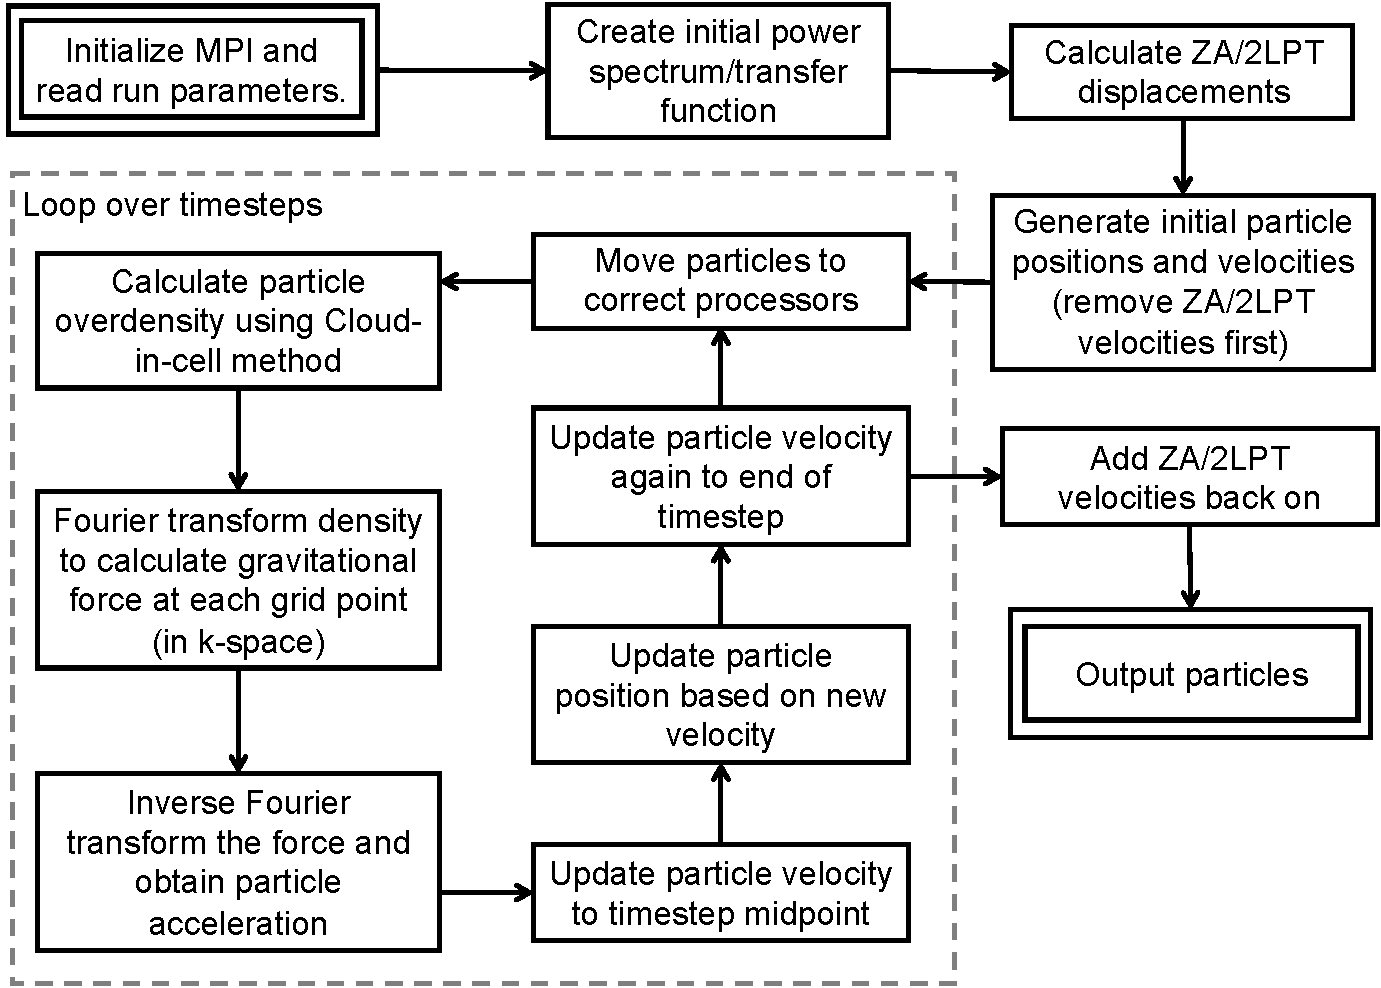
\includegraphics[width=0.8\textwidth]{PICOLAchart.pdf}
  \caption{A simple flowchart of the steps {\sc picola} takes in generating a dark matter realisation from scratch. The blue box indicates where the inclusion of primordial non-Gaussianity changes the code structure. The red boxes highlight areas where the code differs depending on whether we are running snapshot or lightcone simulations \textbf{XXXX: Replace with better figure}.}
  \label{PICOLAchart}
\end{figure*}

\section{Parallelisation}
Parallelisation of {\sc picola} has been performed with the goal that each processor can run a small section of the simulation whilst needing minimal knowledge of the state of the simulation as a whole. We have separated both the mesh and particles across processors in one direction. In this way each processor gets a planar portion of the mesh, and the particles associated with that portion. We have tried to balance the load on each processor as much as possible while observing the fact that each processor must have an integer number of mesh cells in the direction we have split the full mesh. This process is enabled by use of the publicly available MPI-FFTW libraries, which also serve to perform the Fast Fourier Transforms when the mesh is split over different processors\footnote{These are included in the FFTW package mentioned previously}. In a simulation utilising $N_{p}$ processors and consisting of a cubic mesh of size $N_{mesh}^{3}$, each processor gets $(\lceil N_{m}/N_{p} \rceil)$ slices of the mesh where each slice consists of $N_{m}\times 2(N_{m}/2+1)$ cells. The extra $2N_{m}$ cells in each slice are required as buffer memory for the FFTW routines. Depending on the ratio of $N_{m}$ to $N_{p}$ this may give too many slices in total, so then we work backwards, removing a slice from each processor until the correct number of total of slices is equal to $N_{m}$. The number of particles each processor has is related to the number of mesh cells on that processor as each processor only requires knowledge of any particles that interact with its portion of the mesh. Hence, as the particles are originally spaced equally across the mesh cells, each processor initially holds $N^{3}/N_{m}\times(\lceil N_{m}/N_{p} \rceil)$ particles.

All parallelisation in the code use the Message Passing Interface (MPI) library \textbf{XXXX: Include link in footnote}.In the following subsections we detail the three main parallel algorithms in the code: parallel Cloud-in-cell interpolation, parallel FFT's and moving particles between processors.

\subsection{Parallel Cloud-in-cell}

As each processor only contains particles which belong to the mesh cells it has, the density assignment step proceeds as per the standard Cloud-in-cell interpolation method, except near the 'left-hand' edge of the processor. Here the density depends on particles on the preceding processor. Figure \ref{cloudincell} shows a 2-D graphical representation of this problem.

\begin{figure}
\centering
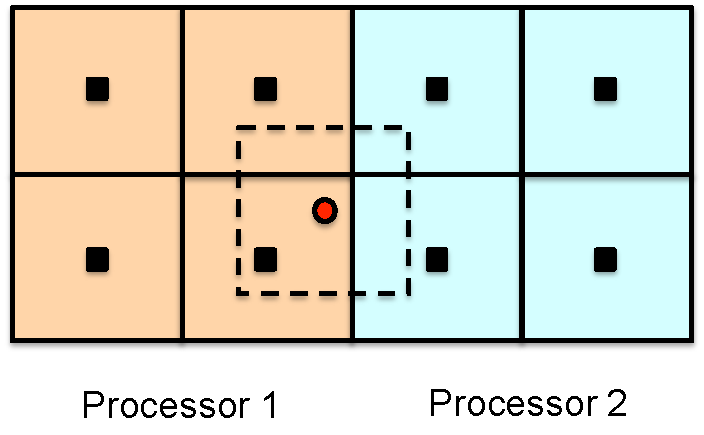
\includegraphics[width=84mm]{cloudincell.pdf}
  \caption{A simple flowchart of the steps {\sc picola} takes in generating a dark matter realisation from scratch. The blue box indicates where the inclusion of primordial non-Gaussianity changes the code structure. The red boxes highlight areas where the code differs depending on whether we are running snapshot or lightcone simulations \textbf{XXXX: Replace with better figure}.}
  \label{cloudincell}
\end{figure}

In order to compensate for this we assign an extra mesh slice to the 'right-hand' edge of each processor. This slice represents the leading slice on the neighbouring processor and by assigning the particles to these where appropriate and then transferring and adding the `slices' to the appropriate processors, each portion of the mesh now contains an estimate of the density which matches the estimate as if all the mesh were contained on a single processor. 

It should also be noted that a reverse of this process must also be done after calculating the forces at each mesh point, as the displacement of a particle near the edge of a processor is reliant on the force at the edge of the neighbouring processor.

\subsection{Parallel FFT's}

To take the Fourier transform of our mesh once it is split over many processors we use the parallel FFTW-MPI routines available alongside the aforementioned FFTW libraries. This is intimately linked to the way in which the particles and mesh are actually split over processes and routines are provided in this distribution that enable us to perform this split in the first place. 

The FFTW routines use a series of collective MPI communications to transpose the mesh and perform a multi-dimensional real-to-complex discrete Fourier transformation of the density, assigning the correct part of the transformed mesh to each process. In terms of implementing this all that is required is for us to partition the particles and mesh in a way that is compatible with the FFTW routines, create a FFTW plan for the arrays we wish to transform and perform the Fourier transformation once we have calculated the required quantity at each mesh point. The FFTW libraries perform all MPI communications and operations internally.

\subsection{Moving Particles}

One final modification to the Particle-Mesh algorithm is to compensate for the fact that over the course of the simulation particles may move outside the physical area contained on each processor, and their position may now correspond to a portion of the mesh that the process in question does not have. This is showly pictorally in Figure \ref{moveparticles}. As such, after each timestep we check to see which particles have moved outside the processor boundaries and move them to the correct processor. This is made particularly important as the COLA method converges in very few timesteps, meaning the particles can move large distances in the space of a single step. 

\begin{figure}
\centering
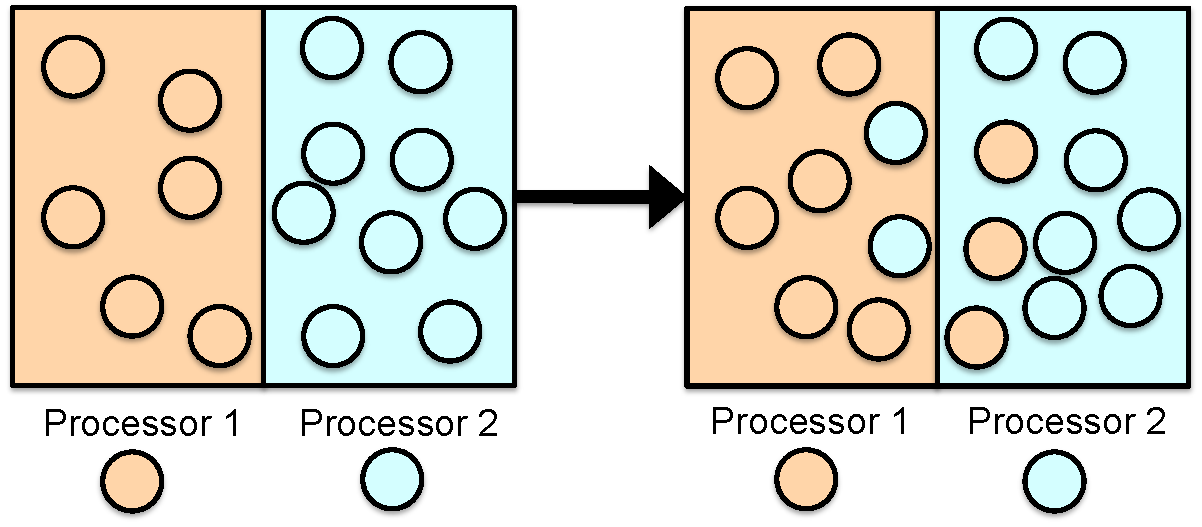
\includegraphics[width=84mm]{moveparticles.pdf}
  \caption{A simple flowchart of the steps {\sc picola} takes in generating a dark matter realisation from scratch. The blue box indicates where the inclusion of primordial non-Gaussianity changes the code structure. The red boxes highlight areas where the code differs depending on whether we are running snapshot or lightcone simulations \textbf{XXXX: Replace with better figure}.}
  \label{moveparticles}
\end{figure}

In the case where we have a high particle density or small physical volume assigned to each process, a single particle can jump across several neighbouring process in a single timestep. So, when moving the particles, we iterate over the maximum number processes any single particle has jumped moving all the particles that have moved to the neighbouring process first, then all particles that have moved to the neighbouring process+1 and so on.

As the simulation progresses the particles will not remain homogeneously spread over the processes, so we assign additional buffer memory to each process to hold any extra particles it acquires. This is utilised during the moving of the particles and all particles a process receives are stored in this buffer. However, in order to make sure this buffer is not filled too quickly we also use the fact that each process is likely to lose some particles and so when a particle is identified as having left a particular process the particle is moved into temporary memory and the gap is filled with a particle from the end of the processes main particle memory. In this way we collect all remaining particles together before moving the new particles across, ensuring a contiguous, compact particle structure. This is shown in Figure \ref{moveparticles2}

\begin{figure}
\centering
\includegraphics[width=84mm]{moveparticles2.pdf}
  \caption{A simple flowchart of the steps {\sc picola} takes in generating a dark matter realisation from scratch. The blue box indicates where the inclusion of primordial non-Gaussianity changes the code structure. The red boxes highlight areas where the code differs depending on whether we are running snapshot or lightcone simulations \textbf{XXXX: Replace with better figure}.}
  \label{moveparticles2}
\end{figure}

\section{Generating Initial Conditions}
In order to allow PICOLA to run a simulation from scratch we have integrated an initial conditions generator into the code. This means that we can simply store the first and second order Lagrangian displacements for each particle as they are calculated rather than assume some initial positions for the particles and reconstruct them. We use the latest version of the parallelised 2LPTic code \cite{Scoccimarro2010} to generate the initial conditions, with some modifications to allow a more seamless combination of the two codes, especially in terms of  parallelisation. For compatibility with PICOLA we have removed the warm dark matter and non-flat cosmology options from the 2LPT initial conditions generator, though these are improvements that could easily be added in the future. The initial positions of the particles are assumed to be at mesh points so rather then creating the particles at this stage, we also conserve memory by generating the 2LPT displacements at mesh points and creating the particles just before timestepping begins.

\textbf{XXXX: Marc, do you want to put some stuff in here about generating IC's from an initial power spectrum?}

Because of this addition, PICOLA can be used very effectively to create the initial conditions for other N-Body simulations, as well as evolving the dark matter field itself. In fact in a single run we can output both the initial conditions and the evolved field at any number of redshift between the redshift of the initial conditions and the final redshift, which allows easy comparison between PICOLA and other N-Body codes.

A final point is that because the 2LPT section is based on the latest version of the 2LPTic code, we are also able to generate, and then evolve, initial conditions with local, equilateral, orthogonal or generic primordial non-gaussianity. Local, equilateral and orthogonal non-gaussianity can be added simply by specifying the appropriate option and providing a value for $F_{NL}$. We can also create primordial non-Gaussianity for any generic bispectrum configuration using a user-defined input kernel, as defined in the Appendix of \cite{Scoccimarro2012}.

\textbf{XXXX: Marc, can you add to this?}

\section{Lightcone}
The final large modification we have made to the code, and one which will be very useful for future large scale structure surveys, is the ability to generate lightcone simulations in a single run, as opposed to running a large number of snapshots and piecing them together afterwards.

Snapshot simulations, generated at some effective redshift, have been widely used in the past to calculate the covariance matrix and perform systematic tests on data, however as future surveys begin to cover larger and larger cosmological volumes with high completeness across all redshift ranges the effect of simulating variable clustering as a function of redshift, which mimics the observations more closely, becomes more and more important. As has been done in several studies \textbf{XXXX: list of references...}, we can piece together a set of snapshot simulations at different redshifts to create a more realistic simulation, however this requires significant post-processing and storage space than generating a lightcone simulation at run-time. As such, in order to provide a useful tool for future cosmology surveys, we have implemented the latter into {\sc picola}.

This is done as follows: The user specifies an initial and final redshift for the lightcone they wish to simulate and an origin, the point at which the observer sits. If we imagine the lightcone as shrinking towards the origin as the simulation progresses, then for every timestep between these two redshifts we can output only those particles that have left the lightcone. If particles have left the lightcone we interpolate the exact time they exited the lightcone,
\begin{equation}
a_{L} = a_{i}+\frac{(a_{i+1}-a_{i})(R_{L,i}-R_{part,i})}{(R_{p,i+1}-R_{p,i})-(R_{L,i+1}-R_{L,i})}.
\end{equation}
Here, $R_{L}$ is the radius of the lightcone at the beginning or end of the timestep. $R_{p}$ is the distance between the origin and the particle. Once we know the exact time the particle left the lightcone we can update the particle's position, using Eq. (A13), to the position it had when it left the lightcone and output the particle. The simulation then continues as normal. We do not interpolate the velocity, using instead the velocity from the previous interation, as is done for the Kick-Drfit-Kick method anyway.

This whole procedure can be performed with minimal extra runtime, as we simply modify the Drift part of the code. Here we need to calculate the position the particle moves to during the current timestep anyway, so the only extra computations are to check the particle's new position against the lightcone and interpolate if necessary. In fact in some cases lightcone simulations are actually faster than snapshot simulations as we are able to output the particles in stages, as they leave the lightcone, rather than creating a bottleneck when all the particles are output at the same time at the end of the simulation.

\textbf{XXXX: Some sort of diagram here.}

\subsection{Replicates}

On top of the standard lightcone interpolation we have accounted for the fact that lightcones built from snapshots simulations often replicate the simulation output to reach the desired redshift. {\sc picola} has the ability to replicate the box as many times as required in each direction during runtime. This is done by simplying modifying the position of each particle as if it was in a simulation box centred at some other location. In this way we can build up a large cosmological volume whilst still retaining a reasonable mass and force resolution, at the expense of some shared large scale modes and covariance. This is done in such a way as to add no additional memory requirements to the run, however the amount of time to drift the particles will increase proportionally to the number of replicates. 

In order to speed this up we identify, each timestep, which replicates are necessary to loop over. Any replicates that have all 8 vertices inside the lightcone at the end of the timestep will not have particles leaving the lightcone and so can be ignored for the current iteration. Furthermore, for replicates not fully inside the lightcone, we calculate the shortest distance between the replicate and the origin by first calculating the distance to each face of the replicate then the shortest distance to each line segment on that face. If the shortest distance to the origin is larger than the lightcone radius then the replicate has completely exited the lightcone and will no longer be required for the duration of the simulation. Overall, this means that even if the simulation box is replicated $N$ times in each direction we will only need to look at a small fraction of the replicates ($\sim1-2$ in each direction unless the simulation box is so small that the lightcone radius changes by more than the boxsize in a single timestep).

\textbf{Show 2D dark matter field with obvious replicates.}

\subsection{Comparison of snapshots and lightcone}

\textbf{It would be cool to compare the halos from snapshots and lightcones and also, if possible, the effect on the covariance matrix. We could then also look at the cross covariance between replicated patches.}

\section{Comparison to N-Body simulations and 2LPT}

\subsection{Accuracy}

\textbf{Comparisons of 2LPT, PICOLA and GADGET. These have probably already been done.}

\subsection{Speed}

\textbf{Would be good to look at speed/scaling between 2LPT, PICOLA and GADGET to show that PICOLA is only a little slower than 2LPT but much, much faster than GADGET}

\section{Discussion and Improvements}

\section{Conclusion}
What have we been talking about? \\
What are the main results? \\
 - Summarise them. \\
What are the main points for the future? 

\begin{thebibliography}{99}

\bibitem[Bouchet et 
al.(1995)]{Bouchet1995} Bouchet, F.~R., Colombi, S., Hivon, E., \& Juszkiewicz, R.\ 1995, A\&A, 296, 575 

\bibitem[\protect\citeauthoryear{Fukugita et al.}{1996}]{F}  Fukugita, M., Ichikawa, T., Gunn, J.~E., Doi, M., Shimasaku, K.,  Schneider, D.~P., 1996, AJ, 111, 1748

\bibitem[Klypin 
\& Holtzman(1997)]{1997astro.ph.12217K} Klypin, A., \& Holtzman, J.\ 1997, arXiv:astro-ph/9712217 

\bibitem[Moutarde et al.(1991)]{Moutarde1991} Moutarde, F., Alimi, 
J.-M., Bouchet, F.~R., Pellat, R., \& Ramani, A.\ 1991, ApJ, 382, 377 

\bibitem[Scoccimarro(1998)]{Scoccimarro1998} Scoccimarro, R.\ 1998, 
MNRAS, 299, 1097 

\bibitem[Tassev et al.(2013)]{Tassev2013} Tassev, S., Zaldarriaga, 
M., \& Eisenstein, D.~J.\ 2013, JCAP, 6, 36 

\end{thebibliography}

\end{document}